This section aims to integrate both the role of the noun in the sentence as well as the role of pragmatic cues like perceptual context and world knowledge for relative adjective interpretation, presenting the \textbf{reference-predication trade-off hypothesis} of comparison class inference. 

Specifically, the issue of comparison class determination is approached from a functional perspective, based on the question what \emph{informational goals} speakers might pursue when producing an utterance containing an adjective, and how these goals might influence listeners’ comparison class inferences \parencite{tessler2020}.
The proposed approach is an inferential account of comparison class determination, informed by the idea of recursive social reasoning mechanisms, applied to rational language use in a Gricean tradition: Speakers have certain informational goals which guide how they craft their utterance in order to facilitate message interpretation with respect to these particular goals for a listener \parencite{goodman2016}. Listeners, in turn, infer the most likely state of the world---that is, in case of gradable adjectives, the most likely comparison class---in light of those speaker goals. 

In particular, in contrast to cases considered in eye-tracking studies described in Chapter \ref{chapter02},  when using adjectives speakers might also primarily intend to convey a property of a target referent. In order to communicate that property of a referent, speakers must achieve at least two informational goals: \textit{reference}---identifying the right target---and \textit{predication}---attributing a property to the target, which in case of relative gradable adjectives amounts to communicating the specific degree of the feature denoted by the adjective \parencite{Reboul2001, Kennedy2007}.  
For these two informational goals, it is reasonable to posit that listeners generally expect the subject to be sufficient in order to establish reference---independent of the predicate asserted to hold of the subject \parencite{Reboul2001, syrett2010meaning, searle1969speech}. Cooperative speakers then aim to satisfy this general expectation.

This tendency is particularly strong for sentences with subjects containing referential expressions like definite descriptions, pronouns or deictics (cf. Section \ref{2.4.}). Furthermore, it might be based on general information structural reasons: In order to predicate a property of a target, this target must be clear \parencite{searle1969speech, krifka2008basic}. Therefore, the subject also tends to convey the \textit{topic} of an utterance---that is, ``the entity [...] under which the information from the comment constituent should be stored" \parencite[p. 265]{krifka2008basic}; while the predicate tends to convey the \textit{comment},  i.e., potentially new information about that entity \parencite{krifka2008basic, chafe1976givenness, Reboul2001}. A further heuristic distinction associated with the subject-predicate contrast comes from linguistic packaging literature wherein the predicate is assumed to convey the \textit{main news} (as opposed to \textit{secondary information}), and also potentially \textit{new information}, while the subject might convey secondary information which is already \textit{known} \parencite{kaiser2020}. 

Note, however, that there are exceptions to many of these tendencies: for instance, for the sentence “The boss fired the worker because he was a convinced communist” the pronominal ``he" can be resolved not only after applying the predicate, but also only taking into account the context---``he" can either refer to the boss or to the worker \parencite{Reboul2001}. \textcite{krifka2008basic} also points out that the topic, and hence the subject,  doesn't necessarily convey known information.
Yet, we posit that these structural expectations are a general enough heuristic holding in many contexts.

These expectations have implications for comparison classes of gradable adjectives insofar as that speakers have the liberty to choose from truth-conditionally similar sentence options to communicate the same message. For example, in order to tell a friend on the phone about a huge dog that the speaker saw today, they have the liberty to say ``That was big!", ``That Great Dane was big!" or ``That was a big dog!", among many other options. Consequently, the choice of a particular sentence over other equivalent options might respond to particular informational-communicative needs. 
%some 4-year-old kids on a playground in winter that they built a big snowman, a speaker has the liberty to say “That’s big!” pointing at the snowman, “That snowman you built is big!” or “You built a big snowman!”, among many other options. Consequently, the choice of a particular sentence over other equivalent options might respond to particular informational - communicative needs. 

From this perspective, the influence of the noun on the comparison class in a simple \textit{Subject Predicate} sentence depends on its position in the sentence. If the noun appears in the predicate of the sentence (e.g., in “That’s a big Great Dane”), it can naturally be explained as produced by a speaker intending to constrain the comparison class, by packaging the noun along with the adjective as the most important information. By contrast, if the noun appears in the subject of the sentence (e.g., in “That Great Dane is big”), it can potentially be \emph{explained away} as produced by a speaker who intends it to support reference (especially via combining it with the deictic ``that"), and hence the noun is a weaker cue towards the comparison class. The comparison class inference is then guided by other pragmatic cues like world knowledge or perceptual context (Fig. \ref{model-cartoon}).

\begin{figure*}[t]
	\begin{center}
		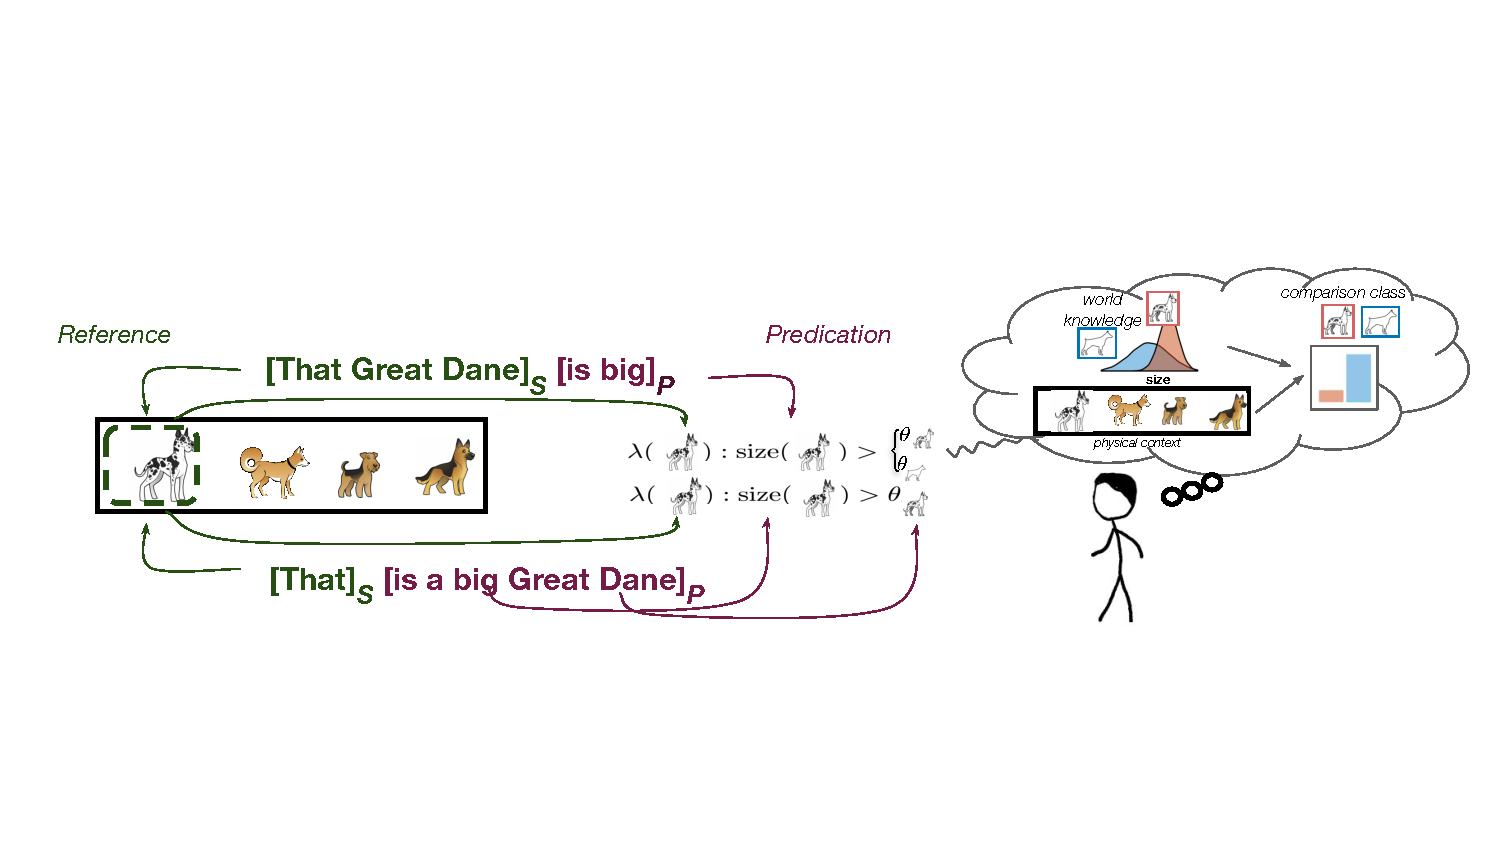
\includegraphics[width=0.9\linewidth]{screenshots/model-cartoon.pdf}
	\end{center}
	\vspace{-2cm}
	\caption{Cartoon of the inferential account for comparison class determination. The noun (Great Dane) in a sentence can be employed either for the goal of reference (green) or predication (purple), shown in the case when this distinction is made via the syntactic position of the noun (subject S~vs.~predicate P). When the noun is used for reference (top), a listener is left with uncertainty about what to use as the comparison class (dogs or Great Danes) and integrates their world knowledge and the physical context to make this inference.  When the noun is used for predication (bottom), the listener should have less uncertainty about the comparison class: The comparison class is stipulated by the noun.}
	\label{model-cartoon}
\end{figure*}
 
Hence, the utility of the noun as constraining the comparison class is the result of a trade-off between its utility in reference and predication, such that comparison class inference is guided by integrating syntactic with other contextual cues.

\section{Understanding Reference and Predication}
\label{3.1.}
This reference-predication trade-off hypothesis focuses on two basic informational goals, reference and predication, which have been discussed in a great deal of work in semantics, pragmatics and philosophy of language \parencite{michaelson2019, Reboul2001}.
 
\textcite{searle1969speech} conceptualizes both reference and predication as particular kinds of propositional acts, defining conditions to be fulfilled in order to accomplish them. Of particular importance for accomplishing reference is that the expression intended for reference isolates the target referent for the listener \parencite{searle1969speech}. Studies have shown that speakers are aware of this requirement, and being sensitive to contextual variability, adjust the informativity of their referential expression correspondingly, such that this requirement is satisfied \parencite[e.g.,][]{graf2016animal}. In particular, definite descriptions which prenominal adjectives might be a part of have been the focus of a lot of work on reference, converging on the claim that a singular determiner phrase of the form \emph{the $\phi$} triggers two presuppositions: the \textit{existence} presupposition (i.e., that there is an object satisfying the description $\phi$), and the \textit{uniqueness} presupposition (i.e., that such an object is uniquely identifiable) \parencite{syrett2010meaning, michaelson2019}. These same presuppositions generally also hold for pronouns and demonstratives, but do not for indefinite descriptions of the form \textit{a $\phi$} \parencite{braun2017, Reboul2001}. Therefore, our experimental operationalization focusing on predication employs gradable adjectives in indefinite descriptions (s. Section \ref{3.2.})

The goal of predication builds upon reference, in that one of the requirements for accomplishing predication is that the same sentence contains a reference to the intended target of predication \parencite{searle1969speech, Reboul2001}. Specifically for relative adjectives, predication is tantamount to communicating a particular property degree, and therefore supplying a felicitous comparison class, for the referent under discussion. Accomplishment of the goal of predication is often roughly equated with the syntactic predicate, which notably might consist of a bare predicative gradable adjective, introduced with a copula. Therefore, one might hypothesize that the noun cannot be the only cue to the comparison class, since predication might be accomplished by a bare adjective.

This review does not attempt to resolve the debate on how exaclty reference and predication might be accomplished. But of particular importance for this work is the flexibility of nouns with respect to both informational goals: combining with the deictic ``that", the noun can accomplish reference; but being part of a non-referential expression (e.g., an indefinite description), the noun can also contribute to predication \parencite{Reboul2001}. 

The focus of this work are these two relatively basic informational goals, but clearly there are other communicative uses of adjectives. For example, \textcite{barker2002dynamics} distinguishes between \textit{descriptive} and \textit{meta-linguistic} uses of vague adjectives. The former refers to what so far has been considered \emph{predication} applied to relative adjectives, while the latter refers to giving ``guidance concerning what the prevailing relevant standard" of comparison is for the adjective under discussion \parencite[p. 2]{barker2002dynamics}. That is, the goal in this case is to teach the appropriate use of the vague adjective, given a particular property value in context. Another related goal of adjective use might be conveying a subjective opinion about a property \parencite{kaiser2020}. Interestingly, gradable adjectives have been shown to differ in the degree of subjective content they might convey \parencite{scontras2017subjectivity}. Further investigation of these communicative goals and their relation to reference and predication is left open to future research.

The discussed properties of reference and predication lead to the particular experimental operationalisation of the reference-predication trade-off hypothesis, described in the next section. 

\section{Experimental Operationalization}
\label{3.2.}
In present studies, the flexibility of nouns to contribute to either informational goal leads to the operationalization of the reference-predication trade-off hypothesis via a syntactic manipulation, wherein the noun (N) which combines with the gradable adjective (ADJ) appears either in the subject or in the predicate of a sentence. Experiments 1--3 employ sentences including only one critical noun N \parencite{tessler2020}:
\begin{quotation}
	\textit{Subject N}: That N is ADJ. 
	
	\textit{Predicate N}: That's a ADJ N.
\end{quotation}
Experiment 4 focuses on the critical noun N1 syntactically modified by the adjective, which then appears either in the subject or in the predicate of an utterance \parencite{TesslerEtAl2020AMLaP}: 
\begin{quotation}
	\textit{Subject N}: That ADJ N1 is a N2. 
	 
	\textit{Predicate N}: That N2 is a ADJ N1.
\end{quotation} 
Given the referential presupposition of the deictic ``that", subject nouns should be taken as establishing reference.  For the predicate noun condition, reference should be taken as being established by the bare deictic or the second noun N2, respectively. Given the presuppositional nature of definite descriptions, the predicate N conditions were chosen to include an indefinite description, such that the predicate may apply to several members of the context and referential pressure be shifted to the subject of the utterance. Furthermore, in the experimental set-up the referent described by critical sentences was perceptually salient, and the task did not involve direct reference resolution, such that referential pressure was generally lower than in eye-tracking experiments described in Section \ref{2.4.}.

Referential utility is operationalized not only through the syntactic position of the noun, but also via the category of the noun: both \emph{basic-level} and \emph{subordinate} referent labels were used (e.g., a Great Dane might be described by the subordinate noun ``Great Dane" or by the basic-level noun ``dog"). While referential utility depends on the context, more specific nouns---i.e., subordinate labels---have generally higher referential utility than more general ones \parencite{graf2016animal}. 

The critical question addressed by this manipulation is how speakers and listeners treat these syntactic frames, asserting the ADJ of referents for whom they are felicitous given one comparison class, but not another (e.g., a \emph{normal-sized} Great Dane can felicitously be described as ``big" given the comparison class ``dogs", but not ‘Great Danes’). 

The reference-predication trade-off hypothesis predicts that nouns that are more likely to establish reference are less likely to constrain the comparison class. Therefore, when the noun appears in the subject of the utterance, it can be explained away as establishing reference, and hence is a weaker cue towards the comparison class, leaving it open to influences of world knowledge and perceptual context. 

 Conversely, when the noun is taken to contribute to predication, i.e., when it appears in the predicate of the sentence, it is more likely to constrain the comparison class. Therefore, listeners would a priori rather expect this noun to be consistent with the comparison class felicitous in order to describe the target referent: for instance, the basic-level category label would be more appropriate for setting the comparison class when describing a normal-sized Great Dane as ``big" than the subordinate category label. That is, the utterance ``That's a big dog" would be more appropriate than ``That's a big Great Dane" in order to describe a normal-sized Great Dane, because the subordinate category \emph{Great Danes} is generally a large-subordinate category compared to the basic-level category \emph{dogs}, but normal-sized representatives are not necessarily large compared to their subordinate category. 

Note that although the differences in comparison class restriction are approached through the lense of this syntactic manipulation, the underlying communicative goals are the primary driving force in comparison class inference, to which the syntax is just a cue. 
There might well be other syntactic realisations of these informational goals (Reboul, 2001): The sentence “What is big is that Great Dane” seems appropriate in a context where generally big things are discussed; in this utterance reference is accomplished from the predicate, and because of this referential pressure, under the trade-off hypothesis the noun would not be expected to constrain the comparison class, although it appears in the predicate, supporting the view that the syntactic position of the noun is dissociable from the intended communicative goals.

To show that informational goals are primary for comparison class inference as opposed to specific syntactic properties of the adjectival phrase, Experiment 4 focuses on manipulating the informational goal the noun is a cue to, while it is directly syntactically modified by the adjective. This manipulation allows to disentangle the effect of the noun position from the effect of syntactic modification of the noun, which are confounded in experiments 1--3. For example, critical sentences in Experiment 4 are “That big Great Dane is a prize-winner” (subject-N) or “That prize-winner is a big Great Dane” (predicate-N). The trade-off hypothesis predicts that even directly modified nouns in the subject position contribute to reference, and thus should be less likely to constrain the comparison class, compared to nouns appearing in the predicate.

The next chapter presents results of these four behavioural experiments exploring the reference-predication trade-off hypothesis, specifically investigating the use of the size adjectives ``big" and ``small". These two adjectives are chosen for practical reasons: size is a visually accessible feature, allowing for easy presentation and manipulation of the context in web-based experiments. Furthermore, humans usually have strong expectations about typical size distributions of different natural categories, from which the target referents were sampled for the experiments. Three distinct dependent measures were used to assess the influence of various cues on comparison class inference. %This experimental data provides a comprehensive overview of pragmatic and syntactic effects on comparsion class inference. 